\section{Модель Кэли~--- Клейна плоскости Лобачевского}

\subsection{Аксиома Лобачевского}

Абсолютной геометрией называют систему аксиом Гильберта без аксиомы параллельности: аксиомы принадлежности (I), порядка (II), конгруэнтности (III) и непрерывности (IV)~[2]. Её теоремы верны и в геометрии Евклида, и в геометрии Лобачевского. Геометрия Лобачевского получается, если к аксиомам I--IV добавить отрицание аксиомы параллельности Евклида.

\begin{definition}[аксиома Лобачевского]
На плоскости существуют прямая $a_0$ и не лежащая на ней точка $A_0$, такие, что через $A_0$ проходят по крайней мере две прямые, не пересекающие $a_0$~[1,~2].
\end{definition}

\begin{theorem}[\!\!{[1]}]\label{thm:lv-vsegda}
Для любой прямой $a$ и любой не лежащей на ней точки $A$ через $A$ проходят по крайней мере две прямые, не пересекающие $a$.
\end{theorem}
\begin{proof}
Допустим, что через $A$ проходит единственная прямая $h$, не пересекающая $a$. Опустим перпендикуляр $AB$ на $a$; перпендикуляр к $AB$ в точке $A$ не пересекает $a$, поэтому совпадает с $h$. Возьмём на $a$ произвольную точку $C$ и отложим от луча $AC$ в полуплоскости, не содержащей $B$, угол $CAM$, равный углу $ACB$. Прямая $AM$ не пересекает $a$ (иначе внешний угол треугольника был бы равен внутреннему, не смежному с ним), поэтому $AM=h$. Тогда сумма углов прямоугольного треугольника $ABC$ равна $\angle B+\angle C+(\angle BAM-\angle CAM)=\pi/2+\angle C+\pi/2-\angle C=\pi$. По второй теореме Лежандра (теорема~\ref{thm:lezhandr2}) отсюда следует аксиома Евклида, что противоречит аксиоме Лобачевского.
\end{proof}

Если $h_1$ и $h_2$~--- две прямые, проходящие через $A$ и не пересекающие $a$, то любая прямая через $A$, лежащая внутри одного из вертикальных углов, образованных $h_1$ и $h_2$ и не содержащих $a$, тоже не пересекает $a$. Поэтому таких прямых бесконечно много.

\subsection{Модель}

Зафиксируем на евклидовой плоскости единичную окружность $\omega$ с центром $O$ и будем называть её \emph{абсолютом}. Следуя~[1,~3], назовём \emph{π-точками} внутренние точки круга, \emph{π-прямыми}~--- хорды без концов, а отношение «π-точка $B$ лежит между $A$ и $C$» определим как то же отношение на евклидовом отрезке. Отношение принадлежности и отношение «между» совпадают с евклидовыми, поэтому аксиомы групп I и II в модели выполнены. Аксиомы непрерывности выполнены потому, что они выполнены на евклидовых отрезках~[1].

Для дальнейшего удобно записывать точки однородными координатами $X=(x_0:x_1:x_2)$, где точке $k=(k_1,k_2)$ плоскости отвечает $X=(1:k_1:k_2)$. Уравнение абсолюта принимает вид $-x_0^2+x_1^2+x_2^2=0$. Его левой части соответствует симметричная билинейная форма
\begin{equation}\label{eq:forma}
\sk{X}{Y}=-x_0y_0+x_1y_1+x_2y_2,
\end{equation}
которую мы будем называть \emph{формой абсолюта}. Точка $X$ лежит внутри круга, если $\sk{X}{X}<0$, на абсолюте, если $\sk{X}{X}=0$, и вне круга, если $\sk{X}{X}>0$.

\begin{definition}
\emph{Полярой} точки $P$ относительно абсолюта называется прямая $\{X:\ \sk{X}{P}=0\}$, а $P$~--- \emph{полюсом} этой прямой.
\end{definition}

Прямая $a_0+a_1k_1+a_2k_2=0$ имеет полюс $P=(-a_0:a_1:a_2)$. Из курса проективной геометрии~[3,~7] известно: поляра внешней точки~--- прямая, проходящая через точки касания двух касательных, проведённых из этой точки к абсолюту; поляра точки абсолюта~--- касательная в этой точке; поляра внутренней точки не пересекает круг. Следовательно, каждая π-прямая имеет полюс вне круга (или в бесконечно удалённой точке, если хорда~--- диаметр): это точка пересечения касательных к абсолюту в концах хорды. Отношение «полюс~--- поляра» взаимно: точка $X$ лежит на поляре точки $P$ тогда и только тогда, когда $P$ лежит на поляре $X$.

\subsection{π-движения и расстояние}

\begin{definition}[\!\!{[1]}]
\emph{π-движением} называется взаимно однозначное отображение круга на себя, которое переводит хорды в хорды и сохраняет сложное отношение любых четырёх точек одной прямой. π-фигуры называются \emph{равными}, если одна переводится в другую π-движением.
\end{definition}

Отображения круга на себя, переводящие хорды в хорды, являются проективными преобразованиями, сохраняющими абсолют. В однородных координатах они задаются матрицами $M$, для которых $\sk{MX}{MY}=\sk{X}{Y}$~[3]. Примеры: поворот вокруг $O$, симметрия относительно диаметра и \emph{сдвиг вдоль диаметра}
\begin{equation}\label{eq:sdvig}
M_t=\begin{pmatrix}\ch t&\sh t&0\\ \sh t&\ch t&0\\ 0&0&1\end{pmatrix},
\end{equation}
который переводит центр $O=(1:0:0)$ в точку $(\ch t:\sh t:0)$, то есть в точку $(\thh t,\,0)$ круга. Сохранение формы проверяется перемножением: $-(\ch t\,x_0+\sh t\,x_1)^2+(\sh t\,x_0+\ch t\,x_1)^2=-x_0^2+x_1^2$. Комбинируя сдвиги и повороты, можно перевести любую π-точку в центр круга. Проверка аксиом III группы для так определённого равенства фигур проведена в~[1].

\begin{definition}
Длиной отрезка $AB$ в модели называется число
\begin{equation}\label{eq:dlina}
d(A,B)=\tfrac12\bigl|\ln(AB,UV)\bigr|,
\end{equation}
где $U$, $V$~--- концы хорды $AB$, а $(AB,UV)$~--- сложное отношение четырёх точек.
\end{definition}

π-движения сохраняют сложное отношение и переводят концы хорды в концы хорды, поэтому равные отрезки имеют равные длины. Для вычислений удобнее другая запись той же величины.

\begin{proposition}\label{prop:ch}
Если $A$ и $B$~--- π-точки, а $A$, $B$ обозначают также их однородные координаты, то
\begin{equation}\label{eq:ch}
\ch d(A,B)=\frac{|\sk{A}{B}|}{\sqrt{\sk{A}{A}\,\sk{B}{B}}}.
\end{equation}
В координатах круга, при $A=(1:a)$, $B=(1:b)$, это равенство принимает вид $\ch d=\dfrac{1-a\cdot b}{\sqrt{(1-|a|^2)(1-|b|^2)}}$.
\end{proposition}
\begin{proof}
Точки прямой $AB$ имеют однородные координаты $A+tB$, и параметр $t$~--- проективный параметр на этой прямой: точке $A$ отвечает $t=0$, точке $B$ отвечает $t=\infty$. Сложное отношение четырёх точек равно сложному отношению их параметров, поэтому для концов хорды с параметрами $t_1$, $t_2$
\[
(AB,UV)=\frac{t_1-0}{t_1-\infty}:\frac{t_2-0}{t_2-\infty}=\frac{t_1}{t_2}.
\]
Концы хорды лежат на абсолюте, то есть $t_1$, $t_2$~--- корни уравнения $\sk{A}{A}+2t\sk{A}{B}+t^2\sk{B}{B}=0$. Обозначим $\alpha=\sk{A}{A}<0$, $\gamma=\sk{B}{B}<0$, $\beta=\sk{A}{B}$ и $\lambda=|\beta|/\sqrt{\alpha\gamma}$. Неравенство $\lambda\ge1$ следует из того, что уравнение имеет действительные корни. Корни равны $t_{1,2}=\bigl(-\beta\pm\sqrt{\beta^2-\alpha\gamma}\bigr)/\gamma$, их произведение $\alpha/\gamma$ положительно, и
\[
\frac{t_1}{t_2}=\Bigl(\frac{\lambda+\sqrt{\lambda^2-1}}{\lambda-\sqrt{\lambda^2-1}}\Bigr)^{\pm1}=\bigl(\lambda+\sqrt{\lambda^2-1}\bigr)^{\pm2}=e^{\pm2\operatorname{arch}\lambda}.
\]
Отсюда $\tfrac12|\ln(AB,UV)|=\operatorname{arch}\lambda$, что и требовалось. Вторая формула получается подстановкой $A=(1,a)$, $B=(1,b)$ в~\eqref{eq:forma}.
\end{proof}

\begin{corollary}\label{cor:ot-centra}
Расстояние от центра круга до π-точки $k$ равно $\operatorname{arth}|k|$. В частности, точка, удалённая от центра на расстояние $x$, изображается точкой на расстоянии $\thh x$ от $O$.
\end{corollary}

Из следствия видно, почему равные отрезки на рисунке модели выглядят по-разному. Отрезки длины $0{,}5$, отложенные подряд от точки $A$, на рисунке сжимаются к краю круга, и бесконечно много таких отрезков помещается на каждой хорде (рисунок~\ref{fig:lineyka}). В интерактивной модели (приложение~А) это видно в сценах «Модель Кэли~--- Клейна» и «π-движения»: при переносе треугольника к абсолюту длины его сторон и углы на панели остаются прежними, а сам треугольник на рисунке уменьшается.

\begin{figure}[H]
\centering
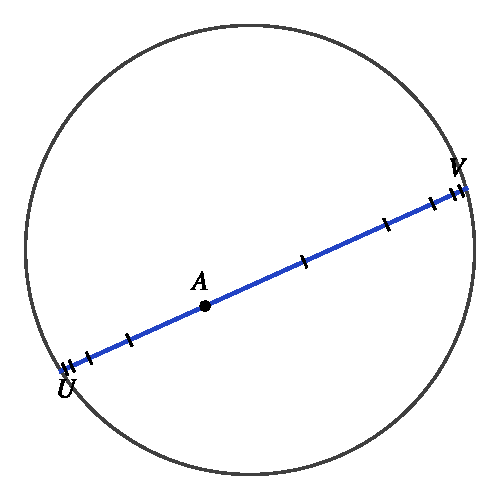
\includegraphics[width=0.46\textwidth]{fig/lineyka.pdf}
\caption{Отрезки длины $0{,}5$, отложенные от точки $A$ в обе стороны по хорде $UV$}
\label{fig:lineyka}
\end{figure}

\subsection{Симметрия относительно прямой и перпендикулярность}

\begin{proposition}\label{prop:simmetriya}
Пусть $\ell$~--- π-прямая, $P$~--- её полюс. Отображение
\begin{equation}\label{eq:otrazhenie}
\sigma_\ell(X)=X-2\,\frac{\sk{X}{P}}{\sk{P}{P}}\,P
\end{equation}
является π-движением, оставляет на месте каждую точку прямой $\ell$, отлично от тождественного и удовлетворяет условию $\sigma_\ell\circ\sigma_\ell=\mathrm{id}$. Это симметрия относительно прямой $\ell$.
\end{proposition}
\begin{proof}
Отображение линейно. Раскрывая скобки, получаем
\[
\sk{\sigma_\ell X}{\sigma_\ell Y}=\sk{X}{Y}-4\frac{\sk{X}{P}\sk{Y}{P}}{\sk{P}{P}}+4\frac{\sk{X}{P}\sk{Y}{P}\sk{P}{P}}{\sk{P}{P}^2}=\sk{X}{Y},
\]
то есть форма абсолюта сохраняется, и $\sigma_\ell$~--- π-движение. Точки прямой $\ell$ удовлетворяют условию $\sk{X}{P}=0$ и остаются на месте. Наконец, $\sigma_\ell(P)=-P$ (та же точка в однородных координатах), и $\sigma_\ell(\sigma_\ell X)=X$ проверяется подстановкой.
\end{proof}

Формула~\eqref{eq:otrazhenie} показывает, что $\sigma_\ell(X)$ лежит на прямой $XP$. Это даёт простое описание перпендикулярности в модели, которое приводится в курсе как построение: перпендикуляр к хорде проводится через её полюс.

\begin{lemma}\label{lem:polyus}
Пусть $m$ и $\ell$~--- π-прямые. Прямая $m$ перпендикулярна $\ell$ тогда и только тогда, когда прямая, содержащая хорду $m$, проходит через полюс $P$ прямой $\ell$.
\end{lemma}
\begin{proof}
Пусть $m$ пересекает $\ell$ в точке $C$. Прямая $m$ перпендикулярна $\ell$ тогда и только тогда, когда она совпадает со своим образом при симметрии $\sigma_\ell$: симметрия переводит угол между $m$ и $\ell$ в смежный с ним, а смежные углы равны только тогда, когда они прямые. Возьмём на $m$ точку $Q\notin\ell$. Образ $\sigma_\ell(Q)$ отличен от $Q$ и лежит на прямой $QP$. Если $P\in m$, то $QP=m$ и $\sigma_\ell(m)=m$. Обратно, если $\sigma_\ell(m)=m$, то $\sigma_\ell(Q)\in m$, и прямая $Q\sigma_\ell(Q)$, совпадающая с $m$, проходит через $P$. Осталось разобрать случай, когда $m$ и $\ell$ не пересекаются. Такие прямые не перпендикулярны по определению. Покажем, что и продолжение хорды $m$ не проходит через $P$.

Каждая хорда, продолжение которой проходит через внешнюю точку $P$, пересекает $\ell$ внутри круга. Действительно, точка, гармонически сопряжённая с внешней точкой $P$ относительно концов любой хорды, проходящей через $P$, лежит на этой хорде и на поляре $\ell$, поэтому каждая такая хорда пересекает $\ell$ внутри круга~[7]. Значит, если $m$ не пересекает $\ell$, её продолжение через $P$ не проходит, и в этом случае обе части утверждения ложны.
\end{proof}

\begin{figure}[H]
\centering
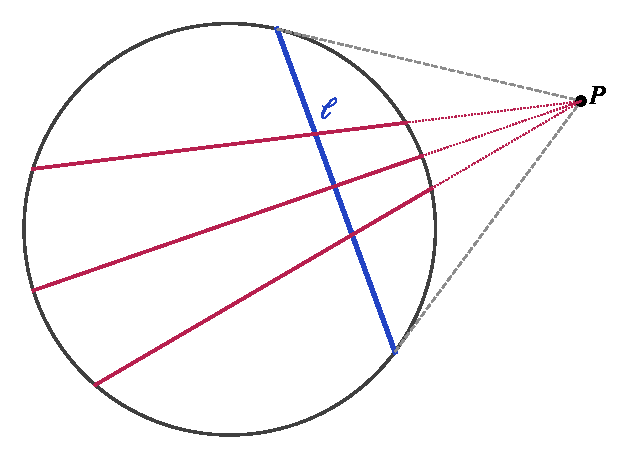
\includegraphics[width=0.5\textwidth]{fig/polyus.pdf}
\caption{Перпендикуляры к π-прямой $\ell$: их продолжения проходят через полюс $P$, точку пересечения касательных к абсолюту в концах хорды $\ell$}
\label{fig:polyus}
\end{figure}

Если $\ell$~--- диаметр, её полюс бесконечно удалён, и лемма говорит, что перпендикуляры к диаметру изображаются хордами, перпендикулярными ему в евклидовом смысле. Этим частным случаем мы будем постоянно пользоваться.

\begin{proposition}\label{prop:ugol}
Пусть π-прямые $\ell_1$ и $\ell_2$ пересекаются, $P_1$ и $P_2$~--- их полюсы, $\varphi$~--- один из углов между ними. Тогда
\begin{equation}\label{eq:ugol}
|\cos\varphi|=\frac{|\sk{P_1}{P_2}|}{\sqrt{\sk{P_1}{P_1}\,\sk{P_2}{P_2}}}.
\end{equation}
\end{proposition}
\begin{proof}
Обе части равенства не меняются при π-движениях, поэтому можно считать, что прямые пересекаются в центре $O$. π-движения, оставляющие $O$ на месте, сохраняют вектор $(1,0,0)$ и форму абсолюта, то есть являются евклидовыми поворотами и симметриями относительно диаметров. Значит, равные углы с вершиной $O$ равны и в евклидовом смысле, а по теореме о единственности меры угла~[2] π-мера угла с вершиной в центре совпадает с евклидовой. Прямые $a_1k_1+a_2k_2=0$ и $b_1k_1+b_2k_2=0$ имеют полюсы $(0:a_1:a_2)$ и $(0:b_1:b_2)$, и правая часть~\eqref{eq:ugol} равна модулю косинуса евклидова угла между нормалями $(a_1,a_2)$ и $(b_1,b_2)$, то есть между самими прямыми.
\end{proof}

Из доказательства видно ещё одно полезное следствие: \emph{угол с вершиной в центре круга изображается без искажения}. Углы с вершиной в другой точке на рисунке искажены, и в интерактивной модели их величина вычисляется по формуле~\eqref{eq:ugol} или, что то же самое, после переноса вершины в центр.
